\documentclass[tikz,border=10pt]{standalone}
\begin{document}
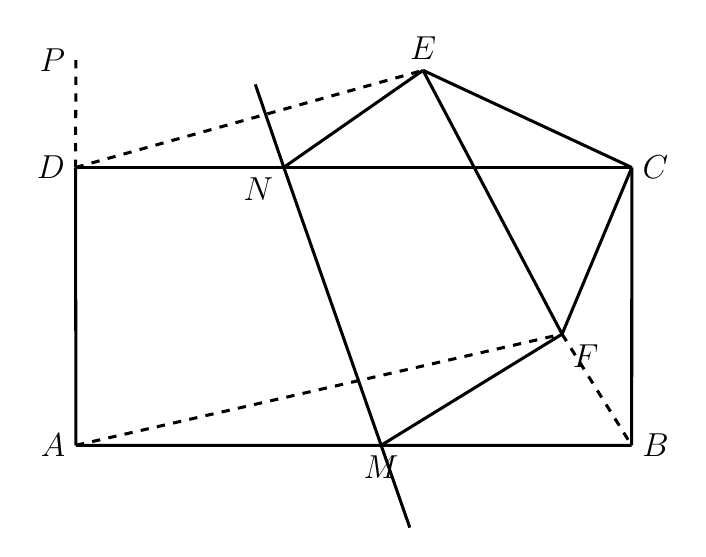
\begin{tikzpicture}[line width=1.1pt, line join=round, font=\fontsize{11.5}{13.8}\selectfont]
\coordinate (A) at (-3.523,-2.118);
\coordinate (B) at (3.535,-2.119);
\coordinate (C) at (3.537,1.410);
\coordinate (D) at (-3.528,1.410);
\coordinate (E) at (0.885,2.644);
\coordinate (N) at (-0.883,1.412);




\coordinate (P) at (-3.523,2.774);   
\coordinate (M) at (0.353,-2.118);   
\coordinate (F) at (2.651,-0.706);   
\coordinate (T) at (-1.245,2.466);   
\coordinate (Q) at (0.717,-3.163);   


\draw (A) -- (B);
\draw (D) -- (C);
\draw (A) -- (D);
\draw (B) -- (C);


\draw[dashed] (P) -- (D);


\draw[dashed] (D) -- (E);
\draw[dashed] (A) -- (F);
\draw[dashed] (F) -- (B);


\draw (C) -- (E);
\draw (E) -- (N);
\draw (E) -- (F);
\draw (F) -- (C);
\draw (M) -- (F);


\draw (T) -- (N) -- (M) -- (Q);


\node[left] at (P) {$P$};
\node[left] at (D) {$D$};
\node[right] at (C) {$C$};
\node[right] at (B) {$B$};
\node[left] at (A) {$A$};
\node[above] at (E) {$E$};
\node[below left] at (N) {$N$};
\node[below] at (M) {$M$};
\node[below right] at (F) {$F$};
\end{tikzpicture}
\end{document}